\documentclass[aspectratio=169, 10pt]{beamer}

% --- Typography & Encodings ---
\usepackage[utf8]{inputenc}
\usepackage[T1]{fontenc}
\usepackage{lmodern}
\usepackage{microtype}
\usepackage{amsmath, amssymb}
\usepackage{booktabs}
\usepackage{listings}

% --- TikZ & Graphics ---
\usepackage{tikz}
\usetikzlibrary{shapes.geometric, arrows.meta, positioning, calc, backgrounds, fit}

% --- Color Palette (Polimi Inspired & Modern Academic) ---
\definecolor{PolimiBlue}{RGB}{0, 43, 73}        % Primary Brand (#002B49)
\definecolor{PolimiLightBlue}{RGB}{0, 119, 182} % Secondary Accent
\definecolor{DarkSlate}{RGB}{33, 37, 41}        % Text
\definecolor{SoftGray}{RGB}{245, 247, 250}      % Background for boxes
\definecolor{AccentOrange}{RGB}{224, 86, 36}    % Warnings & Highlights
\definecolor{AccentGreen}{RGB}{42, 157, 143}    % Success & Quorum

% --- Theme Configuration ---
\usetheme{Boadilla}
\usecolortheme{default}

\setbeamercolor{structure}{fg=PolimiBlue}
\setbeamercolor{palette primary}{bg=PolimiBlue, fg=white}
\setbeamercolor{palette secondary}{bg=PolimiLightBlue, fg=white}
\setbeamercolor{palette tertiary}{bg=PolimiBlue!90, fg=white}
\setbeamercolor{title}{fg=white, bg=PolimiBlue}
\setbeamercolor{frametitle}{fg=white, bg=PolimiBlue}
\setbeamercolor{block title}{bg=PolimiBlue, fg=white}
\setbeamercolor{block body}{bg=SoftGray, fg=DarkSlate}
\setbeamercolor{block title alerted}{bg=AccentOrange, fg=white}
\setbeamercolor{block body alerted}{bg=AccentOrange!10, fg=DarkSlate}
\setbeamercolor{block title example}{bg=AccentGreen, fg=white}
\setbeamercolor{block body example}{bg=AccentGreen!10, fg=DarkSlate}
\setbeamercolor{item}{fg=PolimiLightBlue}

\setbeamertemplate{navigation symbols}{}
\setbeamertemplate{footline}[frame number]
\setbeamertemplate{blocks}[rounded][shadow=true]

% --- Listings Setup for Java & Bash ---
\lstset{
    basicstyle=\ttfamily\scriptsize,
    keywordstyle=\color{PolimiLightBlue}\bfseries,
    stringstyle=\color{AccentOrange},
    commentstyle=\color{gray}\itshape,
    breaklines=true,
    showstringspaces=false,
    backgroundcolor=\color{SoftGray},
    frame=single,
    rulecolor=\color{PolimiBlue!20}
}

% --- Metadata ---
\title[Distributed Job Scheduling]{Distributed Job Scheduling Cluster}
\subtitle{Fault-Tolerant, Load-Balanced Execution Infrastructure}
\author[Distributed Systems Group]{Distributed Systems Project Team}
\institute[Polimi]{
    Politecnico di Milano\\
    \textit{090950 -- Distributed Systems (A.Y. 2025--2026)}\\
    \small Professors: G. Cugola, A. Margara
}
\date{\today}

\begin{document}

% -------------------------------------------------------------
% SLIDE 1: Title Slide
% -------------------------------------------------------------
\begin{frame}[plain]
    \titlepage
\end{frame}

% -------------------------------------------------------------
% SLIDE 2: Core Project Objectives
% -------------------------------------------------------------
\begin{frame}{Core Project Objectives}
    \begin{block}{Project Requirements \& Goals}
        \begin{itemize}
            \item \textbf{Job Submission \& Polling:} Clients submit compute tasks to any node, obtain a unique \texttt{job\_id}, and asynchronously poll for results.
            \item \textbf{Equal Load Sharing:} Executors dynamically balance execution so active load satisfies $|L_i - L_j| \le 1$.
            \item \textbf{Crash-Recovery Model:} Fail-stop and crash-resume (no Byzantine behavior); nodes rejoin seamlessly.
        \end{itemize}
    \end{block}
\end{frame}

% -------------------------------------------------------------
% SLIDE 3: Architectural Constraints & Technologies
% -------------------------------------------------------------
\begin{frame}{Architectural Constraints \& Technologies}
    \begin{exampleblock}{System Design \& Technologies}
        \begin{itemize}
            \item \textbf{Hybrid Communication Stack:}
            \begin{itemize}
                \item \textbf{Java RMI:} Point-to-point RPCs (tasks, results \& votes).
                \item \textbf{UDP Multicast (\texttt{230.0.0.0:4446}):} Decentralized heartbeat gossip and node discovery.
            \end{itemize}
            \item \textbf{Stable Storage:} Disk-based WAL to survive crashes.
            \item \textbf{Code Mobility:} Generic computation via \texttt{SerializableSupplier<T>}.
        \end{itemize}
    \end{exampleblock}
\end{frame}

% -------------------------------------------------------------
% SLIDE 4: System Architecture Overview
% -------------------------------------------------------------
\begin{frame}{System Architecture Overview}

\begin{columns}[T]

% =============================================================
% LEFT COLUMN
% =============================================================
\begin{column}{0.38\textwidth}

\small

\textbf{Layered Distributed Design}

\vspace{0.3cm}

\textcolor{PolimiBlue}{\textbf{Client Layer}}

\begin{itemize}
    \setlength{\itemsep}{0.2em}
    \item Discovers live nodes via \textbf{UDP Multicast}.
    \item Submits \textbf{serializable tasks} through RMI.
    \item Polls task execution status.
\end{itemize}

\vspace{0.2cm}

\textcolor{PolimiBlue}{\textbf{Executor Cluster}}

\begin{itemize}
    \setlength{\itemsep}{0.2em}
    \item \textcolor{AccentOrange}{\textbf{Leader:}}
    coordinates requests and selects the least-loaded executor.

    \item \textbf{Followers:}
    proxy requests, execute jobs and exchange heartbeats.
\end{itemize}

\end{column}


% =============================================================
% RIGHT COLUMN
% =============================================================
\begin{column}{0.60\textwidth}

\centering

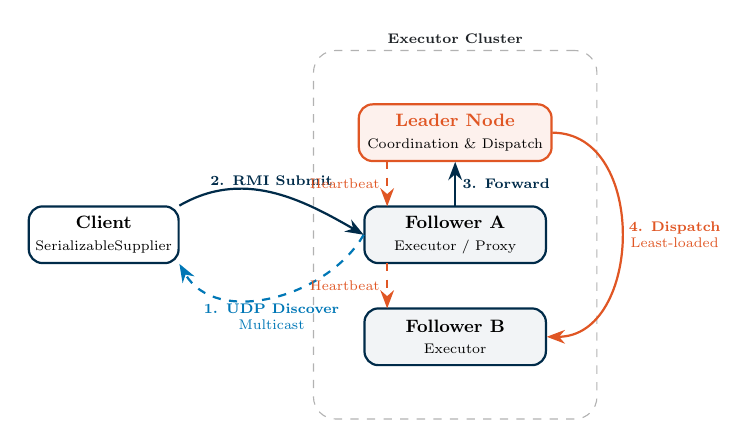
\begin{tikzpicture}[
    scale=0.72,
    transform shape,
    clientbox/.style={
        rectangle,
        rounded corners=5pt,
        draw=PolimiBlue,
        thick,
        fill=white,
        minimum width=2.6cm,
        minimum height=1cm,
        align=center,
        font=\small
    },
    followerbox/.style={
        rectangle,
        rounded corners=5pt,
        draw=PolimiBlue,
        thick,
        fill=PolimiBlue!5,
        minimum width=3.2cm,
        minimum height=1cm,
        align=center,
        font=\small
    },
    leaderbox/.style={
        rectangle,
        rounded corners=5pt,
        draw=AccentOrange,
        thick,
        fill=AccentOrange!8,
        minimum width=3.4cm,
        minimum height=1cm,
        align=center,
        font=\small
    }
]
% -------------------------------------------------------------
% CLUSTER BACKGROUND
% -------------------------------------------------------------
\node[
    draw=gray!60,
    dashed,
    rounded corners=8pt,
    minimum width=5.0cm,
    minimum height=6.5cm
] at (6.2,0) {};
\node[
    font=\scriptsize\bfseries,
    text=DarkSlate
] at (6.2,3.45)
{Executor Cluster};
% -------------------------------------------------------------
% CLIENT
% -------------------------------------------------------------
\node[clientbox] (clientNode) at (0,0)
{
    \textbf{Client}\\
    {\scriptsize SerializableSupplier}
};
% -------------------------------------------------------------
% LEADER
% -------------------------------------------------------------
\node[leaderbox] (leaderNode) at (6.2,1.8)
{
    \textcolor{AccentOrange}{\textbf{Leader Node}}\\
    {\scriptsize Coordination \& Dispatch}
};
% -------------------------------------------------------------
% FOLLOWER A
% -------------------------------------------------------------
\node[followerbox] (followerANode) at (6.2,0)
{
    \textbf{Follower A}\\
    {\scriptsize Executor / Proxy}
};
% -------------------------------------------------------------
% FOLLOWER B
% -------------------------------------------------------------
\node[followerbox] (followerBNode) at (6.2,-1.8)
{
    \textbf{Follower B}\\
    {\scriptsize Executor}
};
% -------------------------------------------------------------
% 1. UDP DISCOVERY
% -------------------------------------------------------------
\draw[
    dashed,
    draw=PolimiLightBlue,
    thick,
    -{Stealth}
]
(followerANode.west)
to[out=240,in=300]
node[
    below,
    midway,
    align=center,
    font=\scriptsize,
    text=PolimiLightBlue
]
{\textbf{1. UDP Discover}\\Multicast}
(clientNode.south east);
% -------------------------------------------------------------
% 2. RMI SUBMIT
% -------------------------------------------------------------
\draw[
    draw=PolimiBlue,
    thick,
    -{Stealth}
]
(clientNode.north east)
to[out=30,in=150]
node[
    above,
    midway,
    font=\scriptsize,
    text=PolimiBlue
]
{\textbf{2. RMI Submit}}
(followerANode.west);
% -------------------------------------------------------------
% 3. FORWARD
% -------------------------------------------------------------
\draw[
    draw=PolimiBlue,
    thick,
    -{Stealth}
]
(followerANode.north)
--
node[
    right,
    midway,
    font=\scriptsize,
    text=PolimiBlue
]
{\textbf{3. Forward}}
(leaderNode.south);
% -------------------------------------------------------------
% 4. DISPATCH
% -------------------------------------------------------------
\draw[
    draw=AccentOrange,
    thick,
    -{Stealth}
]
(leaderNode.east)
to[out=0,in=0,looseness=1.2]
node[
    right,
    midway,
    align=center,
    font=\scriptsize,
    text=AccentOrange
]
{\textbf{4. Dispatch}\\Least-loaded}
(followerBNode.east);
% -------------------------------------------------------------
% HEARTBEAT 1
% -------------------------------------------------------------
\draw[
    dashed,
    draw=AccentOrange,
    thick,
    -{Stealth}
]
(5.0,1.3)
--
node[
    left,
    midway,
    font=\scriptsize,
    text=AccentOrange
]
{Heartbeat}
(5.0,0.5);
% -------------------------------------------------------------
% HEARTBEAT 2
% -------------------------------------------------------------
\draw[
    dashed,
    draw=AccentOrange,
    thick,
    -{Stealth}
]
(5.0,-0.5)
--
node[
    left,
    midway,
    font=\scriptsize,
    text=AccentOrange
]
{Heartbeat}
(5.0,-1.3);
\end{tikzpicture}

\end{column}

\end{columns}

\end{frame}

% -------------------------------------------------------------
% SLIDE 5: Raft-Inspired Consensus
% -------------------------------------------------------------
\begin{frame}{Raft-Inspired Consensus Protocol}
    \begin{block}{Consensus Mechanism (\texttt{ClusterManager})}
        \begin{itemize}
            \item \textbf{States:} \textsc{Follower} $\to$ \textsc{Candidate} $\to$ \textsc{Leader}.
            \item \textbf{Monotonic Epochs (Terms):} Strict epoch counter; stale nodes step down if $\text{term}_{\text{incoming}} > \text{term}_{\text{local}}$.
            \item \textbf{UDP Multicast Heartbeats (3.0s):} Periodic beacon broadcasting node metadata \texttt{(id, ip, port, load, term, isLeader)}.
            \item \textbf{Randomized Election Timeout:} Nodes wait \textbf{5.0--10.0 s} without heartbeat before running for leader (avoids split votes).
        \end{itemize}
    \end{block}
\end{frame}

% -------------------------------------------------------------
% SLIDE 6: Strict Quorum Rule & Configuration
% -------------------------------------------------------------
\begin{frame}{Strict Quorum Rule \& Configuration}
    \begin{alertblock}{Strict Quorum Rule \& Vote Granting}
        \begin{itemize}
            \item \textbf{Vote Request:} Candidate requests votes via RMI \texttt{requestVote(term, candidateId)}.
            \item \textbf{Vote Granting Criteria:} A node votes \texttt{true} if:
            \begin{itemize}
                \item $\text{term}_{\text{candidate}} \ge \text{term}_{\text{local}}$.
                \item The node has not already voted for another candidate in the current term (ensured by the Voter WAL).
            \end{itemize}
            \item \textbf{Quorum requirement:}
            \[
                Q = \left\lfloor \frac{\texttt{expectedClusterSize}}{2} \right\rfloor + 1
            \]
            \item Strict majority intersection guarantees at most one leader per term.
        \end{itemize}
    \end{alertblock}
    
    \vspace{0.1cm}
    \centering
    \scriptsize
    \begin{tabular}{@{}ll@{}}
        \toprule
        \textbf{Parameter} & \textbf{Configured Value} \\
        \midrule
        Heartbeat Interval & 3.0 s (\texttt{UDPMulticastSender}) \\
        Election Timeout & [5.0 s, 10.0 s] (Uniform Random) \\
        Node Eviction Timeout & 15.0 s (\texttt{UDP\_TIMEOUT}) \\
        \bottomrule
    \end{tabular}
\end{frame}
% -------------------------------------------------------------
% SLIDE 7: Job Execution Model & Code Mobility
% -------------------------------------------------------------
\begin{frame}{Job Execution Model \& Code Mobility}
    \begin{columns}[T]
        \begin{column}{0.5\textwidth}
            \begin{block}{Code Mobility via \texttt{SerializableSupplier<T>}}
                \begin{itemize}
                    \item Cluster acts as a Generic Compute Engine (FaaS / Serverless model).
                    \item Client serializes arbitrary Java lambda functions inside \texttt{Job<T>} without modifying server classes.
                \end{itemize}
            \end{block}
            
            \begin{exampleblock}{Least-Loaded Node Dispatching}
                \begin{itemize}
                    \item Leader selects executor with lowest load:
                    \[
                        E_{\text{target}} = \arg\min_{n \in \text{AliveNodes}} (\texttt{n.getActiveJobs()})
                    \]
                    \item Load balanced across fixed thread pools (4 threads/node).
                \end{itemize}
            \end{exampleblock}
        \end{column}
        
        \begin{column}{0.48\textwidth}
            \textbf{End-to-End Execution Pipeline:}
            \begin{enumerate}
                \item \textbf{Ingress:} Client contacts any node $\to$ transparently routed to Leader's RMI stub.
                \item \textbf{Dispatch:} Leader assigns job to least-loaded node $E_{\text{target}}$.
                \item \textbf{WAL Persistence:} $E_{\text{target}}$ writes \texttt{<jobId>.job} to disk before thread execution.
                \item \textbf{Execution:} Worker thread computes lambda result.
                \item \textbf{Result Logging:} Output written to \texttt{<jobId>.result} for polling.
                \item \textbf{Result Retrieval:} Leader scatter-gathers via \texttt{getLocalJobResult(jobId)}.
            \end{enumerate}
        \end{column}
    \end{columns}
\end{frame}

% -------------------------------------------------------------
% SLIDE: Stable Storage: Dual Write-Ahead Log (WAL) - Vertical
% -------------------------------------------------------------
\begin{frame}{Stable Storage: Dual Write-Ahead Log (WAL)}
    \begin{block}{1. Job Compute WAL (\texttt{wal\_<nodeId>/})}
        \begin{itemize}
            \item \textbf{Disk Records:}
            \begin{itemize}
                \item \texttt{<jobId>.job}: Serialized task input.
                \item \texttt{<jobId>.result}: Serialized output.
            \end{itemize}
            \item \textbf{Crash-Recovery Sequence on Boot:}
            \begin{enumerate}
                \item Load all \texttt{*.result} files into memory cache.
                \item Scan \texttt{*.job} files: unfulfilled tasks are automatically re-executed on the thread pool.
            \end{enumerate}
        \end{itemize}
    \end{block}
    
    \vspace{0.15cm}
    
    \begin{alertblock}{2. Raft Voter WAL (\texttt{<nodeId>\_raft.properties})}
        \begin{itemize}
            \item \textbf{Double-Vote Race Condition:} Node votes for candidate A, crashes, restarts in same term, and votes for candidate B $\to$ \textbf{split-brain!}
            \item \textbf{Mitigation:} Synchronously persist \texttt{(currentTerm, votedFor)} to disk before granting any vote (Restored via \texttt{loadRaftState()}).
        \end{itemize}
    \end{alertblock}
\end{frame}

% -------------------------------------------------------------
% SLIDE 9: Network Partitions & Split-Brain Mitigation
% -------------------------------------------------------------
\begin{frame}{Network Partitions \& Split-Brain Mitigation}
    \begin{columns}[c]
        \begin{column}{0.52\textwidth}
            \begin{block}{The \texttt{expectedClusterSize} Invariant}
                \begin{itemize}
                    \item In case of partition $\{S_{\text{maj}}, S_{\text{min}}\}$:
                    \item Fixed \texttt{expectedClusterSize} ($N$) ensures only $S_{\text{maj}}$ can reach majority quorum ($\lfloor N/2 \rfloor + 1$).
                    \item \textbf{Majority Partition ($|S_{\text{maj}}| \ge Q$):} Elects leader, processes jobs, preserves equal load invariant.
                    \item \textbf{Minority Partition ($|S_{\text{min}}| < Q$):} Fails election and remains in \textbf{IDLE / Stalled} state.
                    \item Prevents concurrent rogue leaders and state divergence.
                \end{itemize}
            \end{block}
        \end{column}
        
        \begin{column}{0.46\textwidth}
            \centering
            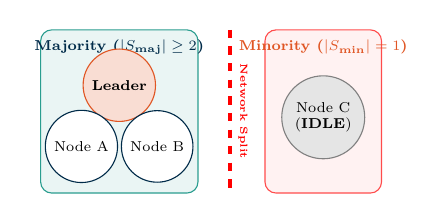
\begin{tikzpicture}[scale=0.74, every node/.style={transform shape}]
                % Majority side
                \node[draw=AccentGreen, fill=AccentGreen!10, rounded corners, minimum width=2.7cm, minimum height=2.8cm] (maj) at (0, 0) {};
                \node[font=\scriptsize\bfseries, color=PolimiBlue] at (0, 1.1) {Majority ($|S_{\text{maj}}| \ge 2$)};
                \node[circle, draw=AccentOrange, fill=AccentOrange!20, font=\scriptsize\bfseries] at (0, 0.45) {Leader};
                \node[circle, draw=PolimiBlue, fill=white, font=\scriptsize] at (-0.65, -0.6) {Node A};
                \node[circle, draw=PolimiBlue, fill=white, font=\scriptsize] at (0.65, -0.6) {Node B};

                % Partition line
                \draw[red, ultra thick, dashed] (1.9, 1.4) -- node[above, sloped, red, font=\tiny\bfseries]{Network Split} (1.9, -1.4);

                % Minority side
                \node[draw=red!70, fill=red!5, rounded corners, minimum width=2.0cm, minimum height=2.8cm] (min) at (3.5, 0) {};
                \node[font=\scriptsize\bfseries, color=AccentOrange] at (3.5, 1.1) {Minority ($|S_{\text{min}}| = 1$)};
                \node[circle, draw=gray, fill=gray!20, font=\scriptsize, align=center] at (3.5, -0.1) {Node C\\(\textbf{IDLE})};
            \end{tikzpicture}
        \end{column}
    \end{columns}
\end{frame}

% -------------------------------------------------------------
% SLIDE 9: Architectural Trade-Offs
% -------------------------------------------------------------
\begin{frame}{Key Architectural Trade-Offs}
    \begin{table}[h]
        \centering
        \scriptsize
        \begin{tabular}{p{2.6cm} p{5.3cm} p{5.5cm}}
            \toprule
            \textbf{Design Dimension} & \textbf{Our Solution} & \textbf{Alternative \& Trade-Off} \\
            \midrule
            \textbf{Partition Handling} & 
            \textbf{Minority stays IDLE} (via \texttt{expectedClusterSize}). Prioritizes consistency and protects equal-load invariant. & 
            \textit{Dynamic Re-clustering:} Minority elects leader; causes split-brain, duplicate execution, and broken load metrics. \\
            \addlinespace
            \textbf{WAL Persistence} & 
            \textbf{Local per-node WAL:} Low latency, zero network overhead; suitable for stateless computational jobs. & 
            \textit{Replicated Global WAL:} High availability during node crashes, but requires heavy distributed consensus per job log. \\
            \addlinespace
            \textbf{Client Discovery \& Routing} & 
            \textbf{Decentralized Multicast Discovery + RMI Proxying:} Client discovers any live node via UDP; Followers transparently route to Leader. & 
            \textit{Dedicated Gateway Proxy:} Centralizes ingress, but introduces a single point of failure (SPOF) and an extra routing hop. \\
            \bottomrule
        \end{tabular}
    \end{table}
\end{frame}
 
% -------------------------------------------------------------
% SLIDE 11: Conclusions
% -------------------------------------------------------------
\begin{frame}{Conclusions \& Key Achievements}
    \begin{columns}[T]
        \begin{column}{0.58\textwidth}
            \begin{block}{Project Summary}
                \begin{itemize}
                    \item \textbf{Hybrid Communication:} Fast RMI point-to-point RPCs combined with UDP Multicast decentralized discovery.
                    \item \textbf{Robust Consensus:} Raft terms, random timeouts (5--10s), and strict quorums prevent split-brain.
                    \item \textbf{Dual WAL Resilience:} Job WAL protects compute tasks; Voter WAL guarantees single-vote election invariant.
                    \item \textbf{Decentralized Architecture:} Direct client multicast discovery and follower transparent forwarding eliminate any single point of failure (SPOF).
                    \item \textbf{Code Mobility:} Generic computation via \texttt{SerializableSupplier<T>}.
                \end{itemize}
            \end{block}
        \end{column}
        
        \begin{column}{0.38\textwidth}
            \centering
            \vspace{0.6cm}
            \Large \textbf{\color{PolimiBlue} Thank you!}\\[0.4cm]
            \includegraphics[width=1.0\linewidth]{foto.png}
        \end{column}
    \end{columns}
\end{frame}

\end{document}